\chapter{Experimental Testing}

\section{Virtual Spring-damper Tests} 
\label{sec:Virtual Spring-damper Tests}
$r_0 = 0.3\ m$\\
$r_{offset} = r - r_0 = 0.13\ m$

\begin{figure}
\centering
\includegraphics[width=1\textwidth]{images/experiments/spring-damper-tests2.eps} 
\caption{Full-leg spring damper testing for radial offset.}
\label{fig:spring-damper-tests}
\end{figure}

Scaling factor of 0.01...
\begin{figure}
\centering
\includegraphics[width=1\textwidth]{images/experiments/joint-spring-damper-tests.eps} 
\caption{Joint spring damper testing for radial offset.}
\label{fig:joint-spring-damper-tests}
\end{figure}

\begin{figure}
\centering
\includegraphics[width=1\textwidth]{images/experiments/full-leg-spring-damper-control-output.eps} 
\caption{Full-leg spring damper motor control.}
\label{fig:full-leg-spring-damper-motor-control}
\end{figure}

\begin{figure}
\centering
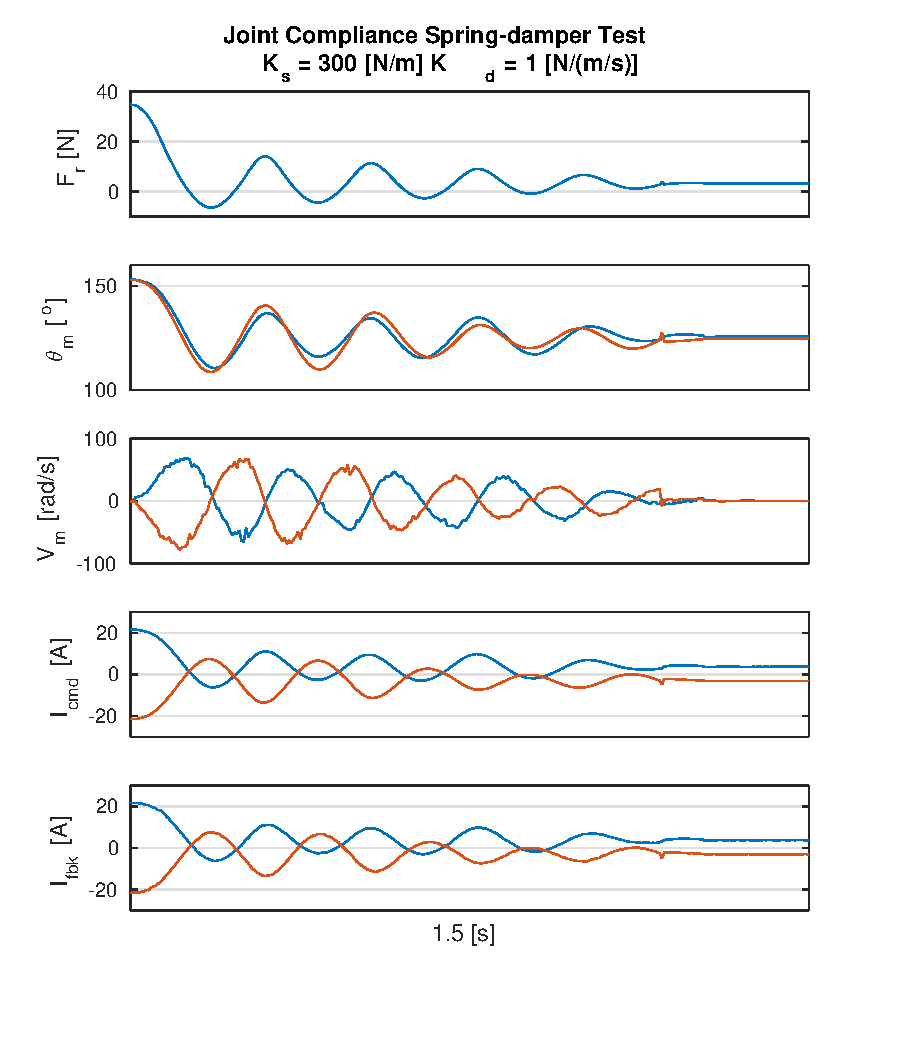
\includegraphics[width=1\textwidth]{images/experiments/joint-spring-damper-control-output.eps} 
\caption{Joint spring damper motor control.}
\label{fig:joint-spring-damper-motor-control}
\end{figure}

\section{Drop Tests}

A theoretical value for the spring constant $K_s$ with $K_d = 5 N/(m/s)$ for radial spring-damping upon impact were determined in \cref{sec:Leg Spring-damper Model} using conservation of energy and an ideal dynamic response. The calculated spring constant of $632.8\ N/m$ was used as a starting point for testing and the damping was varied from $0\ N/(m/s)$ to $5\ N/(m/s)$ to confirm the values derived.

\begin{figure}
\centering
\includegraphics[width=1\textwidth]{images/experiments/drop-test-force-plots.eps} 
\caption{Leg spring damper drop testing.}
\label{fig:drop-tests}
\end{figure}

\section{Launch Tests}

\begin{figure}
\centering
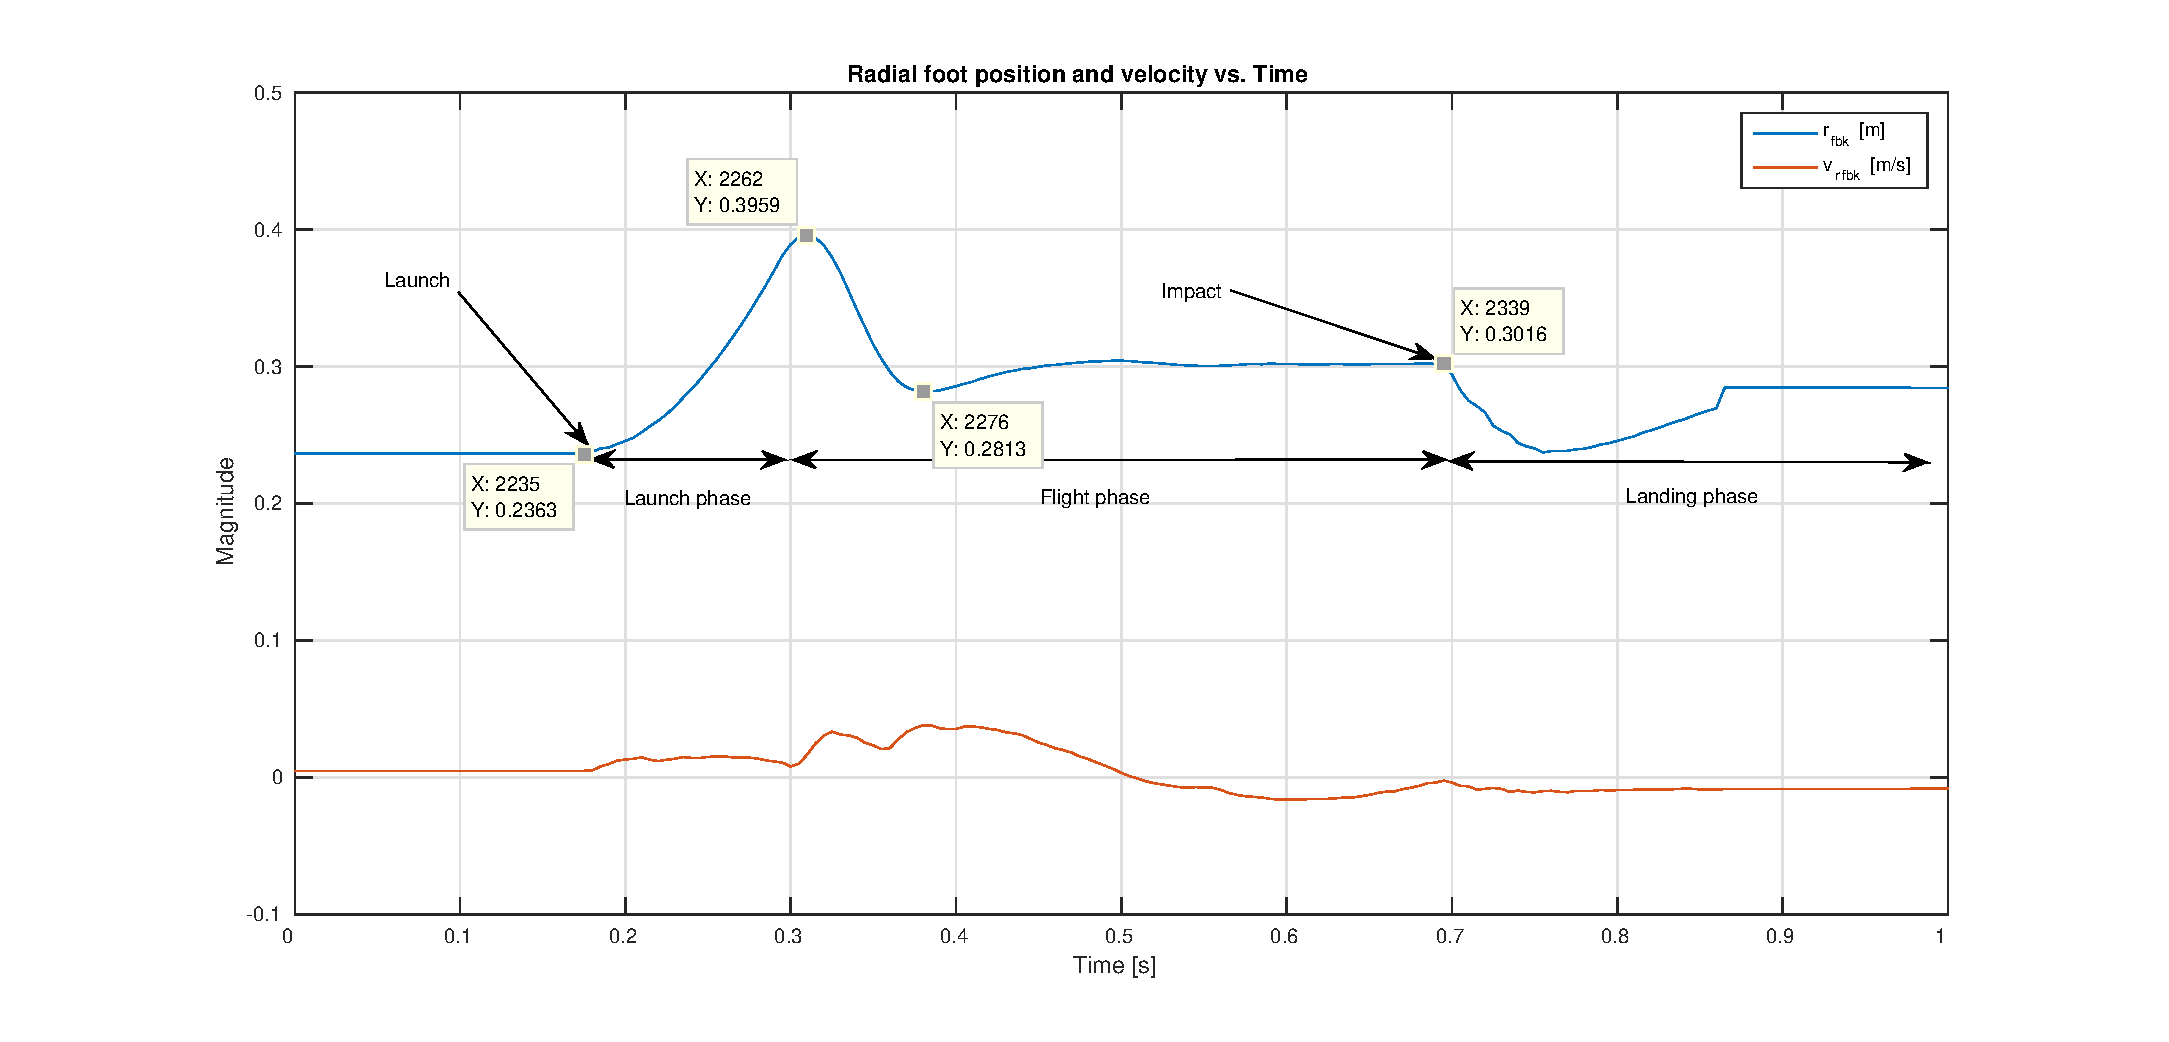
\includegraphics[width=1\textwidth]{images/experiments/jump/jump-foot-position-velocity.eps} 
\caption{Jump foot radial position and velocity (launch and compliant landing).}
\label{fig:Jump foot radial position and velocity}
\end{figure}

\begin{figure}
\centering
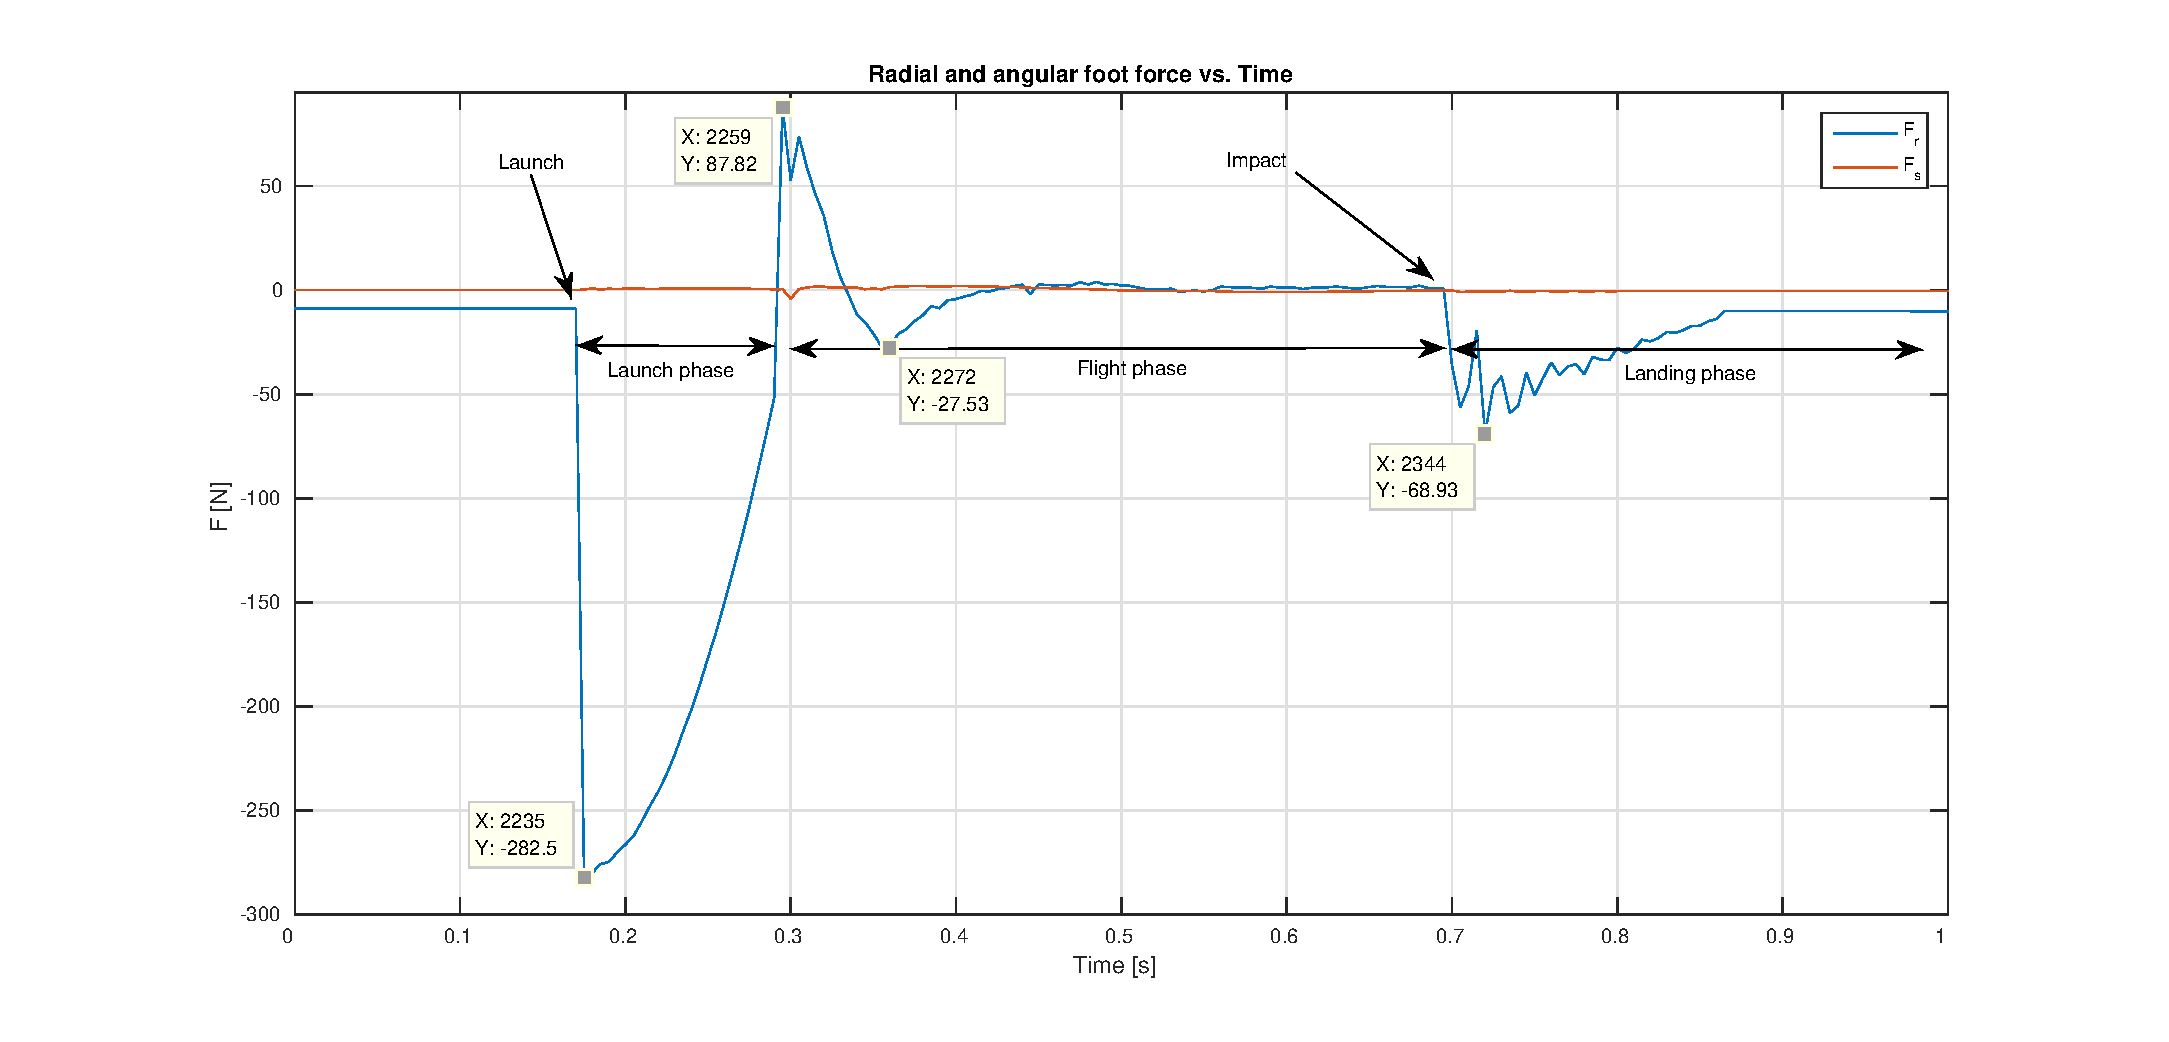
\includegraphics[width=1\textwidth]{images/experiments/jump/jump-foot-force.eps} 
\caption{Jump foot force output (launch and compliant landing).}
\label{fig:Jump foot force output}
\end{figure}

\begin{figure}
\centering
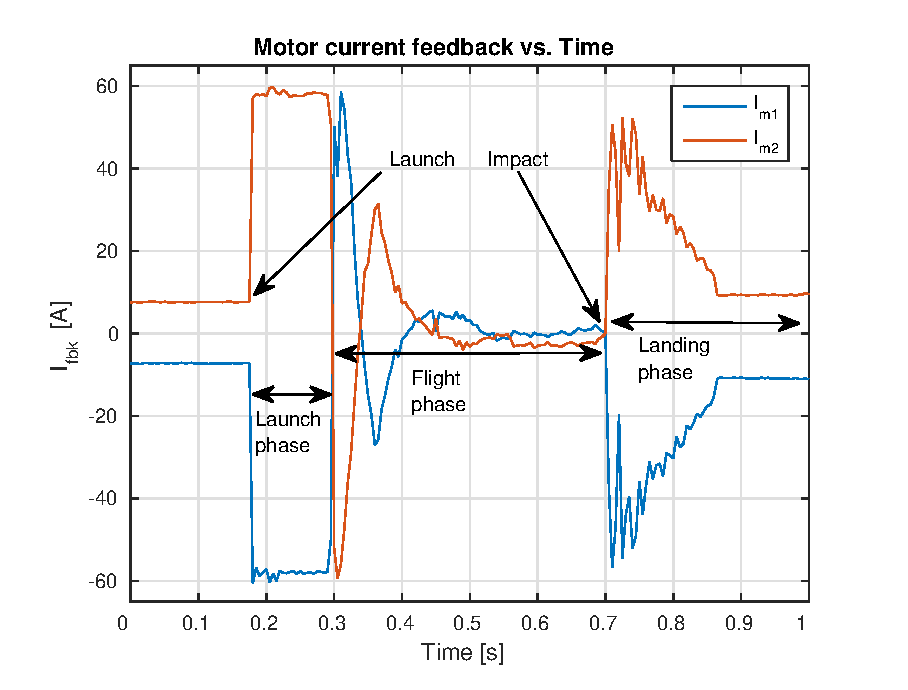
\includegraphics[width=1\textwidth]{images/experiments/jump/jump-current-feedback.eps} 
\caption{Jump motor current feedback (launch and compliant landing).}
\label{fig:jump-motor-current-feedback}
\end{figure}

\begin{figure}
\centering
\subfloat[][Frame 1.]{
\includegraphics[width=0.3\textwidth]{images/experiments/jump/1.png} 
}
\subfloat[][Frame 2.]{
\includegraphics[width=0.3\textwidth]{images/experiments/jump/2.png} 
}

\subfloat[][Frame 3.]{
\includegraphics[width=0.3\textwidth]{images/experiments/jump/3.png} 
}
\subfloat[][Frame 4.]{
\includegraphics[width=0.3\textwidth]{images/experiments/jump/4.png} 
}

\subfloat[][Frame 5.]{
\includegraphics[width=0.3\textwidth]{images/experiments/jump/5.png} 
}
\subfloat[][Frame 6.]{
\includegraphics[width=0.3\textwidth]{images/experiments/jump/6.png} 
}

\subfloat[][Frame 7.]{
\includegraphics[width=0.3\textwidth]{images/experiments/jump/7.png} 
}
\subfloat[][Frame 8.]{
\includegraphics[width=0.3\textwidth]{images/experiments/jump/8.png} 
}

\subfloat[][Frame 9.]{
\includegraphics[width=0.3\textwidth]{images/experiments/jump/9.png} 
}
\subfloat[][Frame 10.]{
\includegraphics[width=0.3\textwidth]{images/experiments/jump/10.png} 
}
\caption{Leg launch with compliant landing.}
\end{figure}

\section{Current Tracking}

\begin{figure}
\centering
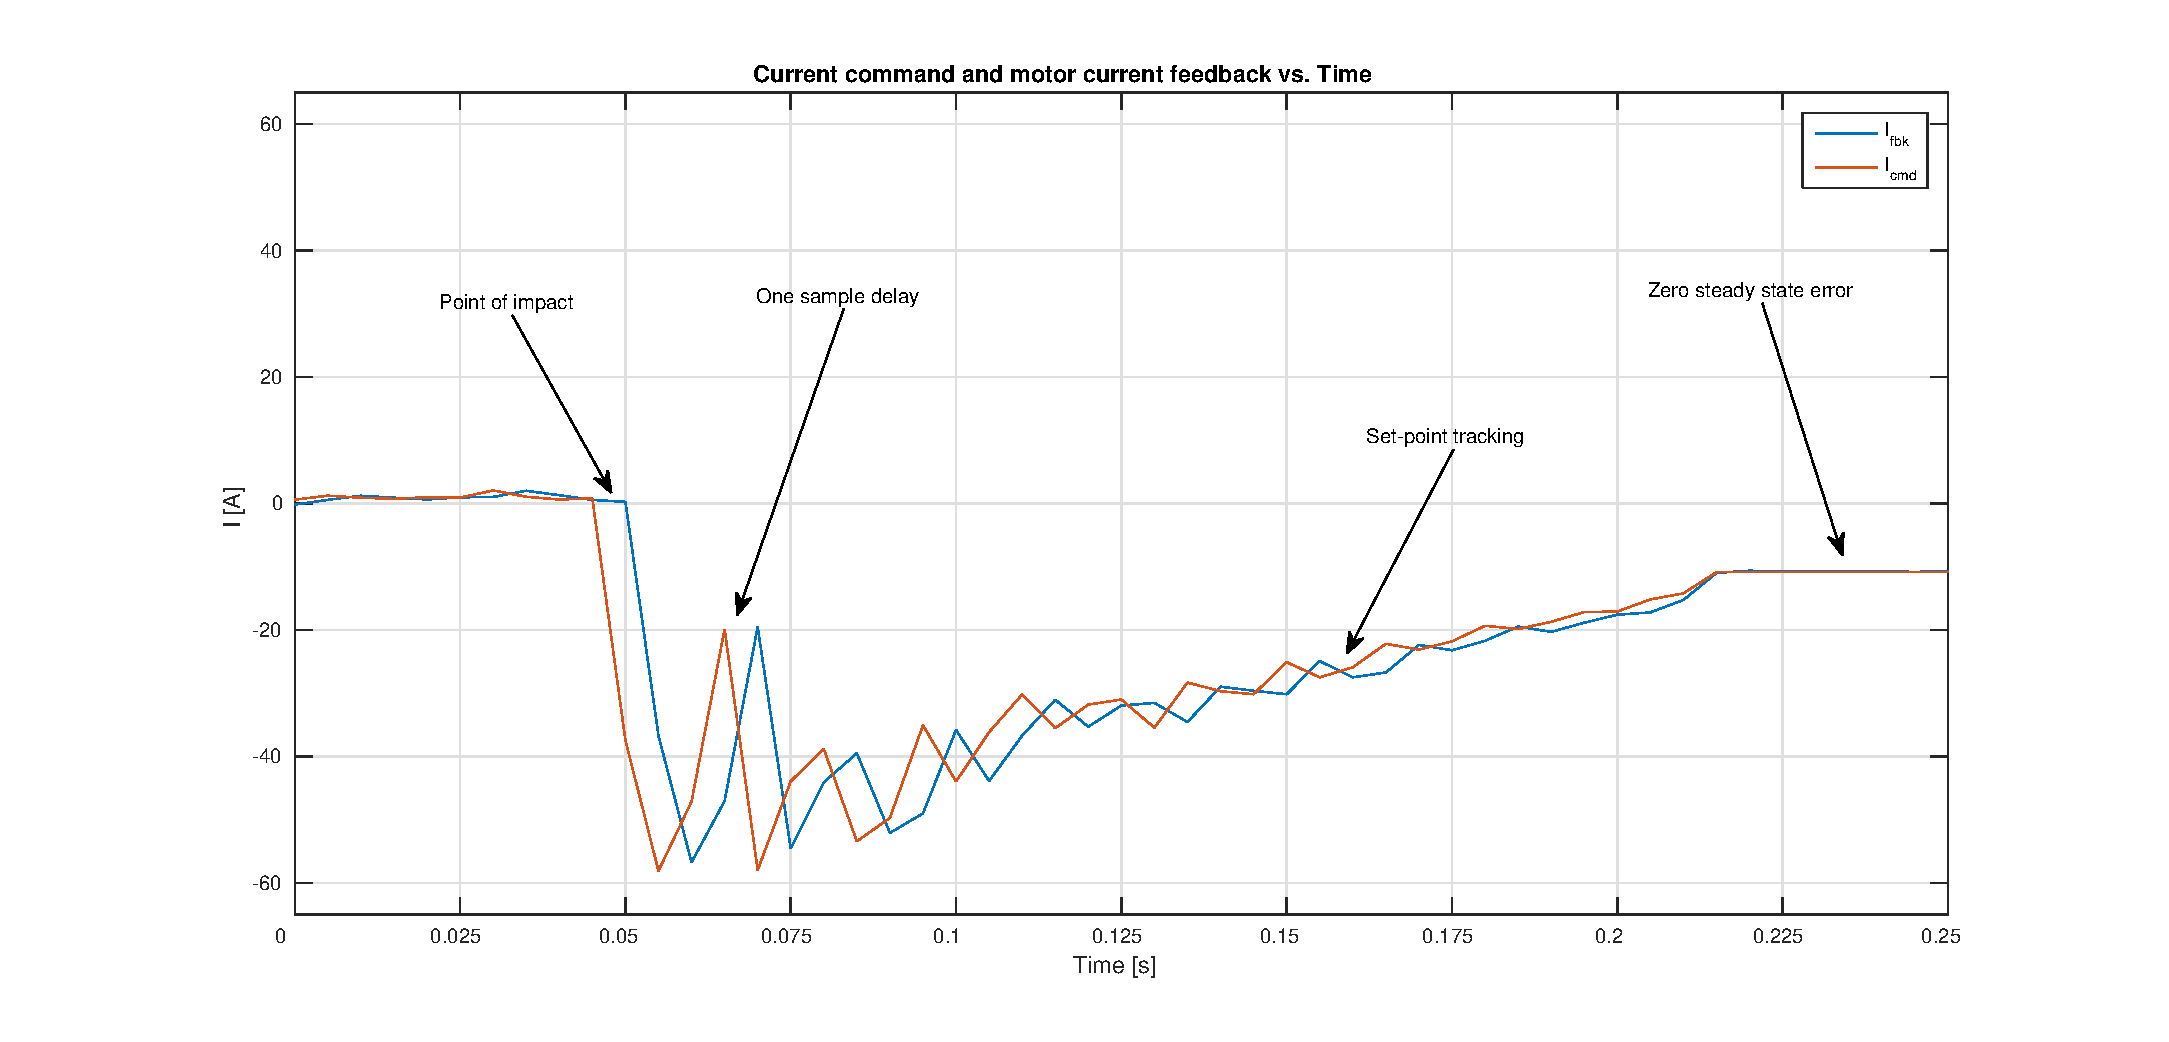
\includegraphics[width=1\textwidth]{images/experiments/current-tracking-impact.eps} 
\caption{Current control tracking.}
\label{fig:Current control tracking}
\end{figure}
